\subsection{Dual-Accumulator Hough Voting}
\label{vote}

Before introducing the instantaneous optimal matching, we first discuss the dual-accumulator Hough voting procedure by which we identify the participants, \textit{i.e.}, compute the best matching matrix $W^{*}$. Note that  $W^{*}$ specifies $N$ targets which demonstrate a consistently similar interactive pattern as the exemplar $\mathcal{D}$ over a substantial period in the input $\mathcal{Q}$. This means that if we `zoom-in' to a temporal unit in this period, say $\mathcal{Q}_{t}$ from the incoming video, and `zoom-in' to a temporal unit, say $\mathcal{D}_{s}$, from the exemplar, the matrix $W^{*}$ should also give the best matching between the two `instantaneous' interactions $\mathcal{Q}_{t}$ and $\mathcal{D}_{s}$. As a consequence, if we compute the optimal matching between the instantaneous interaction $\mathcal{Q}_{t}$ for all $t$ and the instantaneous interaction $\mathcal{D}_{s}$ for all $s$, the same matching $W^{*}$ will emerge many times. In other words, the desired $W^{*}$ will be supported by a large number of optimal instantaneous matchings. 

We denote the optimal matching matrix between instantaneous interactions $\mathcal{Q}_{t}$ and $\mathcal{D}_{s}$ as $W^{t,s}$, and compute a dis-similarity score $D(\mathcal{Q}_{t}, \mathcal{D}_{s})$ which yields a smaller number if the optimal $N$ targets in $\mathcal{Q}_{t}$ better matches with $\mathcal{D}_{s}$ and a larger number otherwise. (The approach to compute them is introduced in Section \ref{agg}.) The scenario now resembles the settings for a general Hough Transform, where the desired parameters are supported by the maximum number of image feature observations: A parameter set and an observation set are established, for every observation one enumerates over all parameters and determines every parameter that is compatible with the observation, the count for that compatible parameter in an accumulator array for all parameters is increased by one, and finally the parameter receiving the maximum number of counts is reported. Here, we regard the parameter set as consisted of two parts - the set of all possible matchings $\mathcal{W}$ and the exemplar $\mathcal{D}$, and we regard the observation set as the input $\mathcal{Q}$. However, note that the overall optimal matching may not simply be achieved on the matching receiving the maximum number of counts, but on the matching which yields the maximum similarity with the exemplar. Therefore, in addition to maintaining an accumulator array for the counts on all matchings $\mathcal{W}$, we also maintain a companion accumulator array for the corresponding dissimilarity measures. 

\begin{figure}[t]
\begin{center}
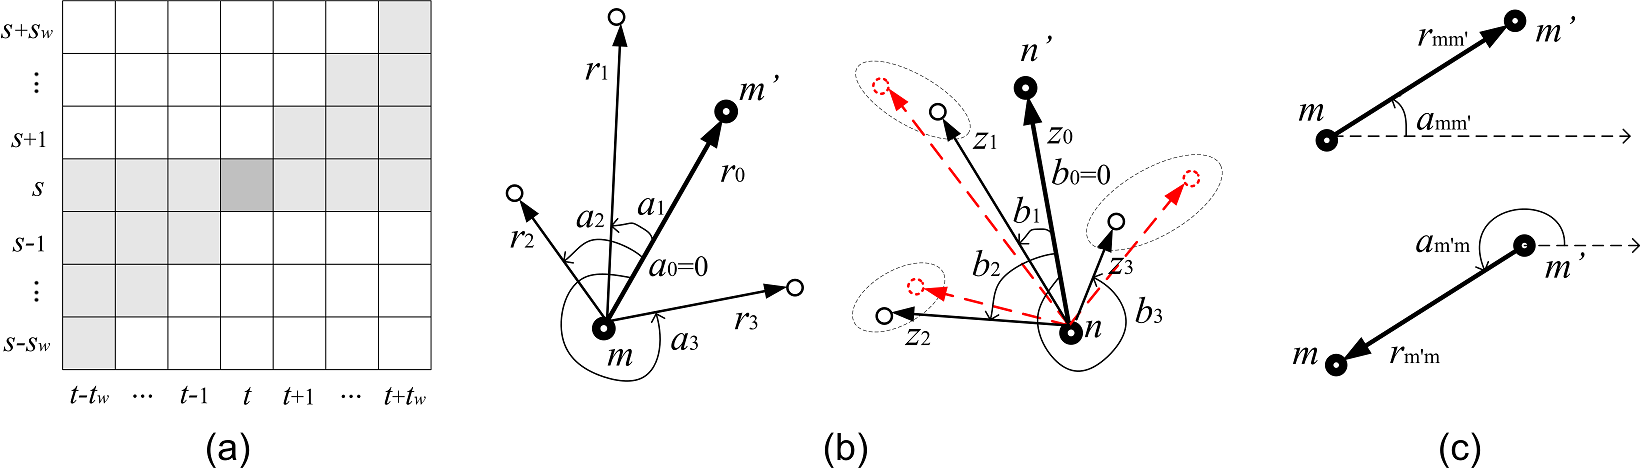
\includegraphics[scale=1.2]{all_illu.png}
\end{center}
\caption{(a) The temporal neighborhood used in to compute \ref{softvote}. See Section \ref{vote} for details. (b) Illustration of the pairwise pairwise descriptors for groups comprised of three or more participants in the classroom interaction database. See Section \ref{expall} for details. (c) Similar illustrations for groups involving only two participants. See Section \ref{expall} for details.}
\label{all_illu}
\end{figure}

Instead of directly using the dissimilarity scores $D(\mathcal{Q}_{t}, \mathcal{D}_{s})$ for the companion array, another fact is that if the matching $W^{t,s}$ is optimal at time pair $(t,s)$, the optimal matchings at the temporally nearby (input, exemplar) time pairs should be also achieved by the same matrix $W^{t,s}$. This means that the matching matrices of these nearby times should all agree, and their dissimilarities $D$'s should all be small. Therefore, we use the follow temporal-consistency preserved dissimilarity measure to vote in the companion array for $W^{t,s}$
\begin{equation}
\label{softvote}
v(W^{t,s})=\sum_{(t',s')\in\mathcal{N}(t,s)}(\|W^{t,s}-W^{t',s'}\|_{1}+1)D(\mathcal{Q}_{t'}, \mathcal{D}_{s'}).
\end{equation}
Here $\mathcal{N}(t,s)$ is a temporal neighborhood of $(t,s)$ in which we enforce the consistency and it is depicted in Figure \ref{all_illu} (a), where the pair $(t,s)$ is shown in black square and the neighborhood is shown in shaded area. Neighborhood sizes $t_{w}$ and $s_{w}$ are taken as a quarter of the length of a cell on the bottom of the pyramid (See Section \ref{BB})\footnote{When the neighborhood extends out of video boundary, we only consider the cells within the boundary and normalize the vote by the number of cells actually involved.}. (\ref{softvote}) implies that, when evaluating the vote $v(W^{t,s})$ for input time $t$ against exemplar time $s$, we also look at the interactive behavior happening ahead of (resp. after) $t$, and expect that the two aforementioned consistencies are maintained so that the the interactive behaviors happening ahead of (resp. after) $t$ resembles that happening ahead of (resp. after) $s$ in the exemplar, in the sense of a smaller $D$ and a same matching matrix. Eventually, a better matching will receive a lower vote. 

\begin{algorithm}
\footnotesize{
\begin{enumerate}
\item Clear both accumulator arrays;
\item For each $t\in[1,T], s\in[1,S]$, increment the count in the cell corresponding to $W^{t,s}$ and increase the vote in the companion array corresponding to $W^{t,s}$ by $v(W^{t,s})$;
\item Identify a subarray of cells receiving more than $\frac{S}{2}$ counts, and normalize the dissimilarity votes in the companion subarray by corresponding counts;
\item Report the matching matrix $W^{*}$ to be the one in the subarray receiving the minimum normalized dissimilarity vote.
\end{enumerate}
}
\caption{\small Dual-accumulator Hough voting procedure for identify the participants (\textit{i.e.}, the best matching $W^{*}$).}
\label{Algo:1}
\end{algorithm}

 As a result, the dual-accumulator Hough voting procedure is shown in Algorithm \ref{Algo:1}, where in the last two steps we find among those matching matrices which receive a substantial number of supports from instantaneous matchings the best matching $W^{*}$ with the lowest average dissimilarity to the exemplar. This idea is also illustrated in Figure \ref{diagram}, where a thick matching line indicates a strong similarity (low vote $v$), and the targets receiving the average lowest votes are selected as participants.


